\documentclass{article}

\usepackage[margin=1in, includefoot]{geometry} % Margins Setup
\usepackage[hidelinks]{hyperref} % Allows for Clickable References

% Graphics Dependencies
\usepackage[]{graphicx} % Allows Image Imports
\usepackage[]{float} % Allows Control of Float Positions
% Table Dependencies
\usepackage{tabulary} % helps with table width formatting and text wrapping in tables
\usepackage[none]{hyphenat} % keeps words from breaking up in tables

% Header/Footer Info
\usepackage[]{fancyhdr} % Header/Footer Setup
\pagestyle{fancy}
\fancyhead{}
\fancyfoot{}
\fancyfoot[R]{\thepage\ }
\renewcommand{\headrulewidth}{0px}
\renewcommand{\footrulewidth}{1px}

\begin{document}
    \begin{titlepage}
        \begin{center}
            \line(1,0){340} \\
            [5mm]
            \huge{\bfseries Correcting Binary Corruption in Matrix Multiplication Using C Programs} \\
            \line(1,0){340} \\
            [.25 in]
            \textsc{\LARGE Gupta College of Science} \\
            \textsc{\LARGE Coastal Carolina University} \\
            [.25 in]
            \textsc{\LARGE Colin Matz \\
            Junior B.S. Information Technology, \\ 
            Cybersecurity Minor \\
            November 23, 2022} \\
        \end{center}
    \end{titlepage}

    % Abstract Page
    \pagenumbering{roman}
    \section*{Abstract}\label{sec:abstract}
    \addcontentsline{toc}{section}{\numberline{}Abstract}
    This is the abstract section for my report.

    \newpage

    % list of Figures/Tables
    \listoffigures
    \addcontentsline{toc}{section}{\numberline{}List of Figures}
    \newpage

    \listoftables
    \addcontentsline{toc}{section}{\numberline{}List of Tables}
    \newpage

    % Table of Contents 
    \tableofcontents
    \thispagestyle{empty}

    % Main Body
    \newpage
    \pagenumbering{arabic}
    \setcounter{page}{1}

    % Actual Paper
    \section{Introduction}\label{sec:intro}
    Blah Blah Blah Blah Blah

    % Test Figure / Example Figure
    \begin{figure}[H]
        \centering
        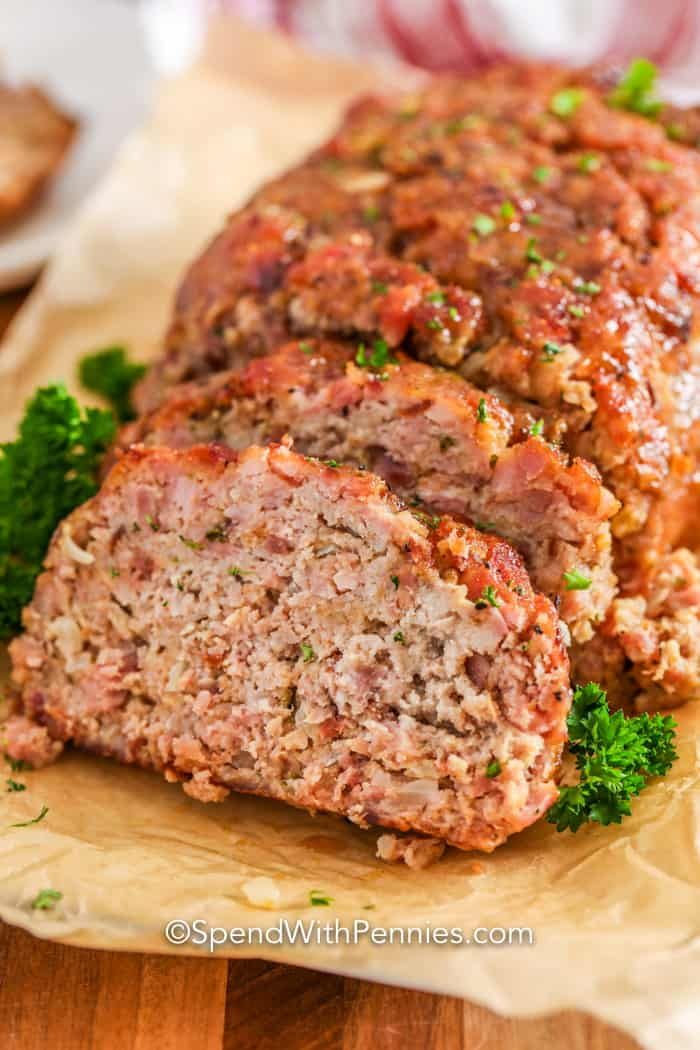
\includegraphics[height=3in]{./media/hamloaf.jpeg}
        \caption[Optional caption]{Real, local caption}
        \label{fig:test}
    \end{figure}

    Figure \ref{fig:test} shows a test image of an hamloaf.

    \section{Related Works}\label{sec:relworks}
    Blah Blah Blah Blah Blah

    \section{Design}\label{sec:design}
    Blah Blah Blah Blah Blah

    \subsection{Structure of Programs}\label{subsec:programstructs}
    Blah Blah Blah Blah Blah

    % test table / example table
    \begin{table}[H]
        \centering
        \caption[Optional Caption]{Real, local caption}
        \label{tab:progsdef}
        \begin{tabulary}{\linewidth}{LCR}
            \hline
            Program Name & Executable Complied & Description of Program \\ 
            \hline
            Test & Test.exe & This program is used in the testing of this table. It uses no parameters but does return 2 values. \\
            Tes2 & Test2.exe & This program is used in the testing of this table. It uses 2 parameters and returns 4 values. \\
        \end{tabulary}
    \end{table}
    
    Table \ref{tab:progsdef} Shows the various programs within my package along with the executables compiled and their uses within the test case.

    \subsection{Functionality at Runtime}\label{subsec:funcrun}
    Blah Blah Blah Blah Blah

    \section{Experiment/Results}\label{sec:ex/res}
    Blah Blah Blah Blah Blah
    \subsection{Testing Environment}\label{subsec:environment}
    Blah Blah Blah Blah Blah
    \subsection{Running the Tests}\label{subsec:runtests}
    Blah Blah Blah Blah Blah
    \subsection{Examining the Results}\label{subsec:examineres}
    Blah Blah Blah Blah Blah

    \section{conclusion}\label{sec:conclusion}
    Blah Blah Blah Blah Blah

    \section{References}\label{sec:refs}

\end{document}